\section{Methods}

\subsection{Model set up}


\subsubsection*{General description}

\begin{figure}[!ht]
    \centering
    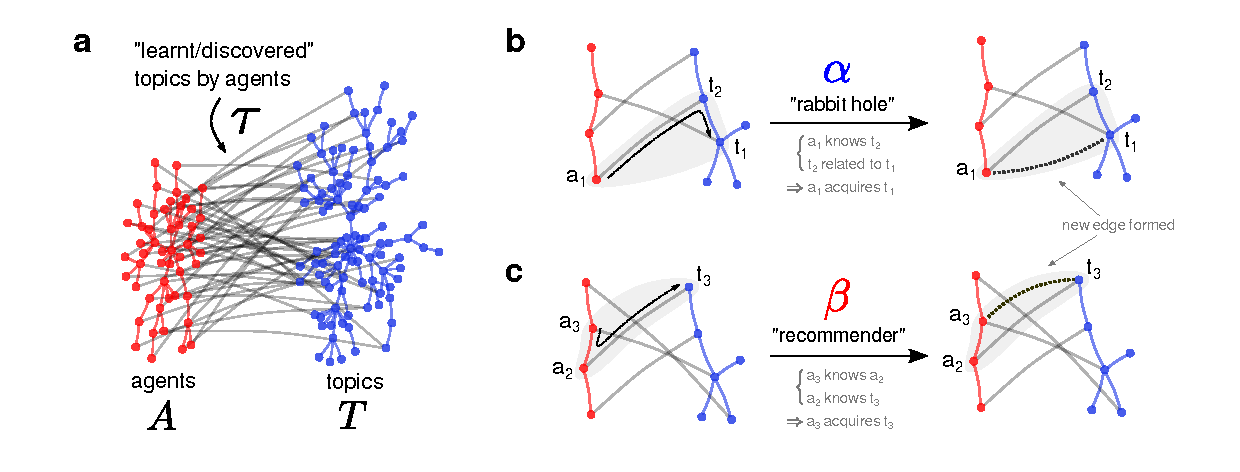
\includegraphics[width=\textwidth]{figures/Fig1.pdf}
    \caption{
    \textit{Model setup and description of the update process}.
    (\textbf{a}) Illustration of the intralayer agent graph (red) and topic graph (blue) with the interlayer edges (gray) representing the knowledge set of the agents.
    (\textbf{b}) and (\textbf{c}) illustrate the update process either through learning/discovery by related topics ("rabbit-hole") or learning/discovery through friends ("recommender")
    }
    \label{fig:1}
\end{figure}

All models considered here are binary undirected graphs. There are $n_a = 200$ agents and $n_t = 1000$ topics. Denote $A$ and $T$ as the symmetric binary adjacency matrices of the agent graph $G_a$ and topic graph $G_t$ respectively (\autoref{fig:1}). The bipartite incidence matrix $\tau$ of size $n_t \times n_a$ represents the topics that the agents know about. It is assumed throughout that the intralayer edges are static while the interlayer edges could be ``acquired" through the update process. And once an interlayer edge is acquired, it is assumed to be persistent. At the initial stage, each agent is assigned at most $\tau_0 = 5$ topics with certain probabilities based on the models of the intralayer models (see below). There is also an upper limit topic capacity $\tau_{\mathrm{max}} = 50$ per agent, and the update process is only simulated until $1.2 \tau_{\mathrm{max}} = 60$ time steps. For each parameter set ($\alpha$, intralayer models, interlayer initialization), I ran 5 simulations each. Hopefully in the future I could acquire more computational resources to run more simulations on larger networks (especially for the more realistic graphs built from real-world networks).

\subsubsection*{Update of interlayer edges}

At each time step, at most one new topic is learnt per agent. The agent could acquire new topic edge either through the ``rabbit-hole'' strategy with $\alpha$ probability, by learning about the related topics of things an agent already knows about. On the other hand, with probability $\beta$, an agent could acquire a new topic edge by traversing its neighbors in the agent graph then to the topic graph. See \autoref{fig:2} for illustration of these processes. One way to implement this is below.

Define $\psi(X)$ as a column L1 normalization operation on a matrix $X$, meaning each column vector $\vec{x}_i$ of the matrix is normalized to $\vec{x}_i/||\vec{x}_i||_1$. Define the shorthand notation for the Heaviside function as $[x]_{\star} = 1$ if $x > 0$, and $0$ otherwise.

At each time step, the probability matrix $P$ (of same size as $\tau$) with its column vector $\vec{p}_i$ defining the probability agent $a_i$ choosing a new topic. A way to define this probability is:

\vspace{-1em}
\begin{align}
    P &=
    {\color{blue}
    \alpha \psi\left(\left[\left[T\tau\right]_{\star} - \tau \right]_{\star}\right)} +
    {\color{red}
    \beta \psi\left(\left[\left[\tau A\right]_{\star} - \tau \right]_{\star}\right)}
    \\
    \tau(t+1) &\leftarrow \tau(t) + \mathrm{sample}(P)
\end{align}

The multiplication steps perform the traversal through neighbors across the intralayer networks. The binarization and subtraction of current $\tau$ simplifies the implementation, to only learn new topics and to balance not being stuck around too popular topics. Additionally, for simplicity here I consider $\beta = 1 - \alpha$ so the process is only defined by $\alpha$. Many other probabilities are ignored as well, for example serendipity (wandering or random discovery of new topics) and forgetting (removal or decrease of strength of interlayer edges). Future implementations should relax these many assumptions for more realistic implementation, and possibly easier to obtain analytical solutions when the nonlinearities are minimized.

\begin{figure}[!ht]
    \centering
    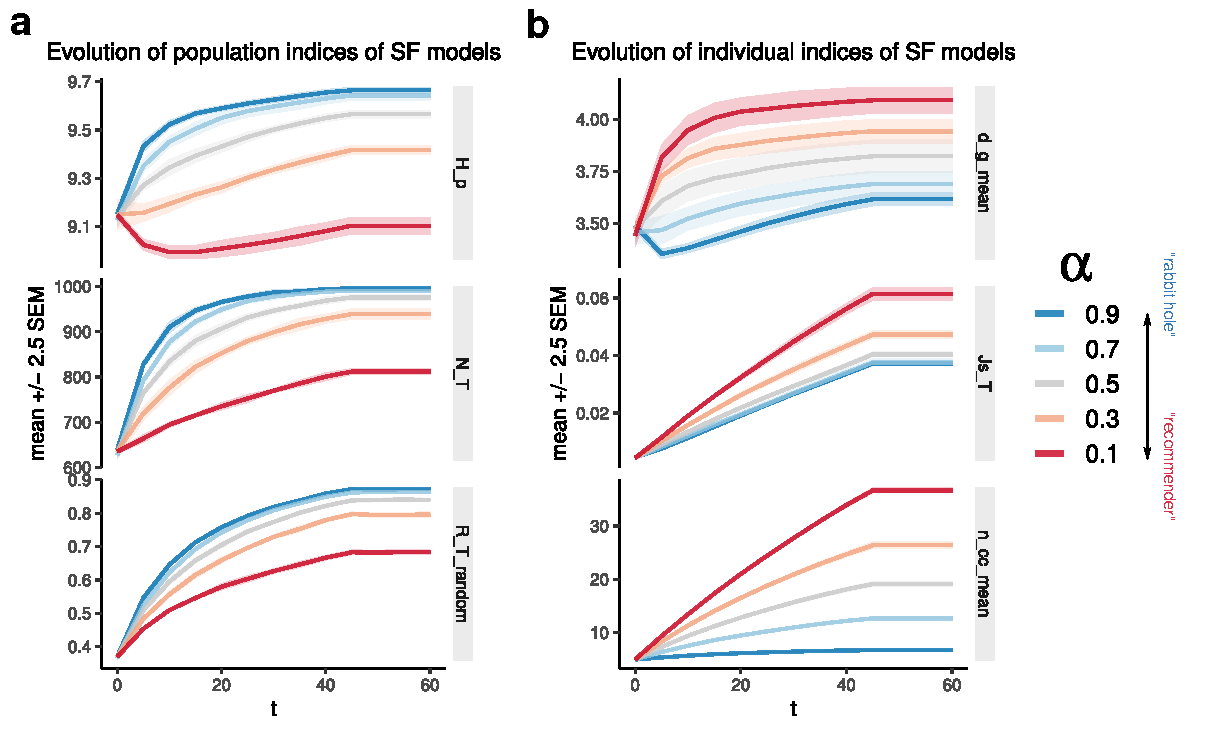
\includegraphics[width=\textwidth]{figures/Fig2.pdf}
    \caption{
    \textit{Changes of population topic diversity indices} (\textbf{a}) \textit{and of individual diversity indices} (\textbf{b}) \textit{of the scale-free (SF) intralayer models} \textit{due to} $\alpha$. $H_p$: topic population entropy; $N_T$: number of distinct topics; $R_T$: robustness due to \textit{random} removal of agents; $d_g$: mean distance of the subset of topics that agents know; $Js_T$: Jaccard similarity of topic set between agents; $n_{cc}$: number of connected components of induced subgraphs based on each agent's learnt topics. See \textbf{Sect. \ref{sec:method-diversity}} and \textbf{Fig. \ref{fig:1}}d,e for more details. Each line represents the mean changes of 5 realizations, analyzed every 5 steps.
    }
    \label{fig:2}
\end{figure}

\subsubsection*{Intralayer random models}

There are different ways to initialize the intralayer networks to match with different empirical results in real social and knowledge networks. For simplicity, the model types and parameters (except only for the number of nodes) are kept the same for agent and topic graphs during each simulation.

\textit{Nonblock models}: The first approach is non-block networks. These include models constructed from preferential attachment models (PA), in which linear PA would lead to a scale-free network with the scaling parameter $\gamma = 3$. I also take into account nonlinear PA models (see \autoref{fig:2}a$_1$). I also include comparison with Erdős–Rényi (ER) networks with different connectivity probability (see \autoref{fig:2}a$_2$), as well as small-world networks generated with the Watts–Strogatz models (see \autoref{fig:2}a$_3$).

\textit{Block models}: Since in real-world networks, there are usually communities (researchers or papers within the same field), I use the stochastic block models (SBM) to emulate this with $k_a = k_t = 10$ groups for both agent and topic networks. A way to manipulate these models is to change the probability of connection within groups ($p_{\mathrm{within}}$) or between groups ($p_{\mathrm{between}}$). For simplicity, I kept the former the same while varying the latter (see \autoref{fig:2}). In retrospect, this makes the models denser by increasing the $p_{\mathrm{between}}$. Future simulations should look for ways to balance this.

Future endeavours should take into account real networks, for example from subsampling a Twitter network as the agent graph and Wikipedia network as the topic graph. Another possibility would be to use citation networks, with authors as agents and papers as topics, groups could be subfields or certain modules in the research topics.

\subsubsection*{Interlayer initialization}

Generally at the initialization stage, the probability of connection between a given agent and topic could be the same across topics. However, it is possible that other initialization strategies might bias the results in one way or another. Hence, I introduce two different interlayer initialization strategies, one for \textit{nonblock} intralayer models and one for \textit{block} models. Whenever an initialization method is not mentioned, it is assumed to be the uniform random strategy.

For \textit{nonblock} intralayer models, the probability of connecting to a certain topic could be dependent on its degree in $G_t$. A way to do this is to perform the $\mathrm{softmax}\left(\{d_i\}; \beta_{\sigma}\right)$ on the degrees, basically transforming the degree sequence $\{d_i\}$ to a probability distribution. With $\beta_{\sigma} < 0$ ($\mathrm{SOFTMAX}_1$), low degrees are favored; $\beta_{\sigma} = 0$ is equivalent to random initialization ($\mathrm{SOFTMAX}_2$), while $\beta_{\sigma} > 0$  ($\mathrm{SOFTMAX}_3$) favors high degree topics (\autoref{supp:1})

For \textit{block} intralayer models, group correspondence could be used as a strategy for initialization as the number of groups are the same for both graphs. This could be parameterized by $p_{\mathrm{sg}}$ (\autoref{supp:2}) as the probability that agents and topics of the same group ID are connected. The chance $p_{sg} = \frac{1}{k_t} = 0.1$ would be equivalent to random initialization.

\subsection{Diversity metric}

\subsubsection*{Population}

Three population indices are defined. First is $N_T$ the number of distinct topics discovered when taking into account all agents' learnt topics (higher would mean more diverse). Second is the topic population entropy $H_p$, which is the Shannon entropy from the discrete probability distribution of all the topics in the population (higher would mean more diverse). Lastly, taken inspiration from ecological bipartitate network stability analysis, robustness can be calculated, by cumulatively removing random agents and observering the number of distinct topics left. The area under this curve is the robustness (higher would mean a lot of agents are needed to be removed to remove a sufficient large proportion of topics).

\subsubsection*{Individual}

Three individual indices are calculated. $d_g$ is the mean distance of the topics in each agent's learnt topics. In other words, if we define $D(t_i,t_j;G_t)$ as the shortest path distance in $G_t$ between $t_i$ and $t_j$, and an agent $a_k$'s topic set as $\tau(a_k)$ then $d_g(a_k) = E\left[D(t_i,t_j;G_t)\right]_{t_i, t_j \in \tau(a_k)}$. Then I take the mean of these distances across off agents of the agent graph. Higher would mean, on average, the agents learn more out of their comfort zone. Another metric is the number connected component $n_{\mathrm{cc}}(a_k)$ of the induced subgraph $G_t(\tau(a_k))$ - higher would mean there are many ``islands'' of topics that the agent knows about, leaning toward generalist trend. Lastly, the pairwise Jaccard similarity between agents' topic sets are calculated $Js_T$, lower would mean higher local diversity on average. Future endeavours should take into account other metrics for local diversity indices (for example local entropies under subsampling of neighbors or nodes within a certain distance).

\subsubsection*{Group}

Additionally, when groups are defined in the block intralayer models, one could also calculate the entropy of the topic group distribution, in both the population sense $H_{\mathrm{gp}}$ and individual sense $H_{\mathrm{gi}}$. More specifically, $H_{\mathrm{gp}}$ is the entropy of the 10 topic groups when taking into account the group identities of all topics learnt by all agents. On the other hand, $H_{\mathrm{gi}}$ is the average entropy of each agent's own topic entropy. These two quantities are different. For example, there could be cases where as a population, $H_{\mathrm{gp}}$ is maximized (all groups uniformly distributed) but $H_{\mathrm{gi}}$ could be 0 (each agent only learns about the topics of the same group, leading individual entropy of 0).